\documentclass{article}
\usepackage[utf8]{inputenc}

\usepackage{graphicx}
\graphicspath{ {Images/} }

\usepackage{authblk}
\usepackage{amsmath}
%\usepackage{titlesec}
\usepackage{caption}
%\addbibresource{references.bib}
\usepackage{geometry}
\usepackage{hyperref}
\usepackage{bold-extra}
\usepackage{enumitem}





\begin{document}
\begin{titlepage}

   \begin{center}
       \vspace*{1cm}


      \Large Programming for Game Engines Assignment 2\\
       \vspace{0.5cm}
       \huge \textbf{A Modular Ability System Implementation in Unreal Engine 5}


            
       \vspace{1cm}
 \Large
     Oliver J. Martin
\\ \large MSc Computer Games
       \vfill
            
       
     \begin{figure}[h]
\centering
       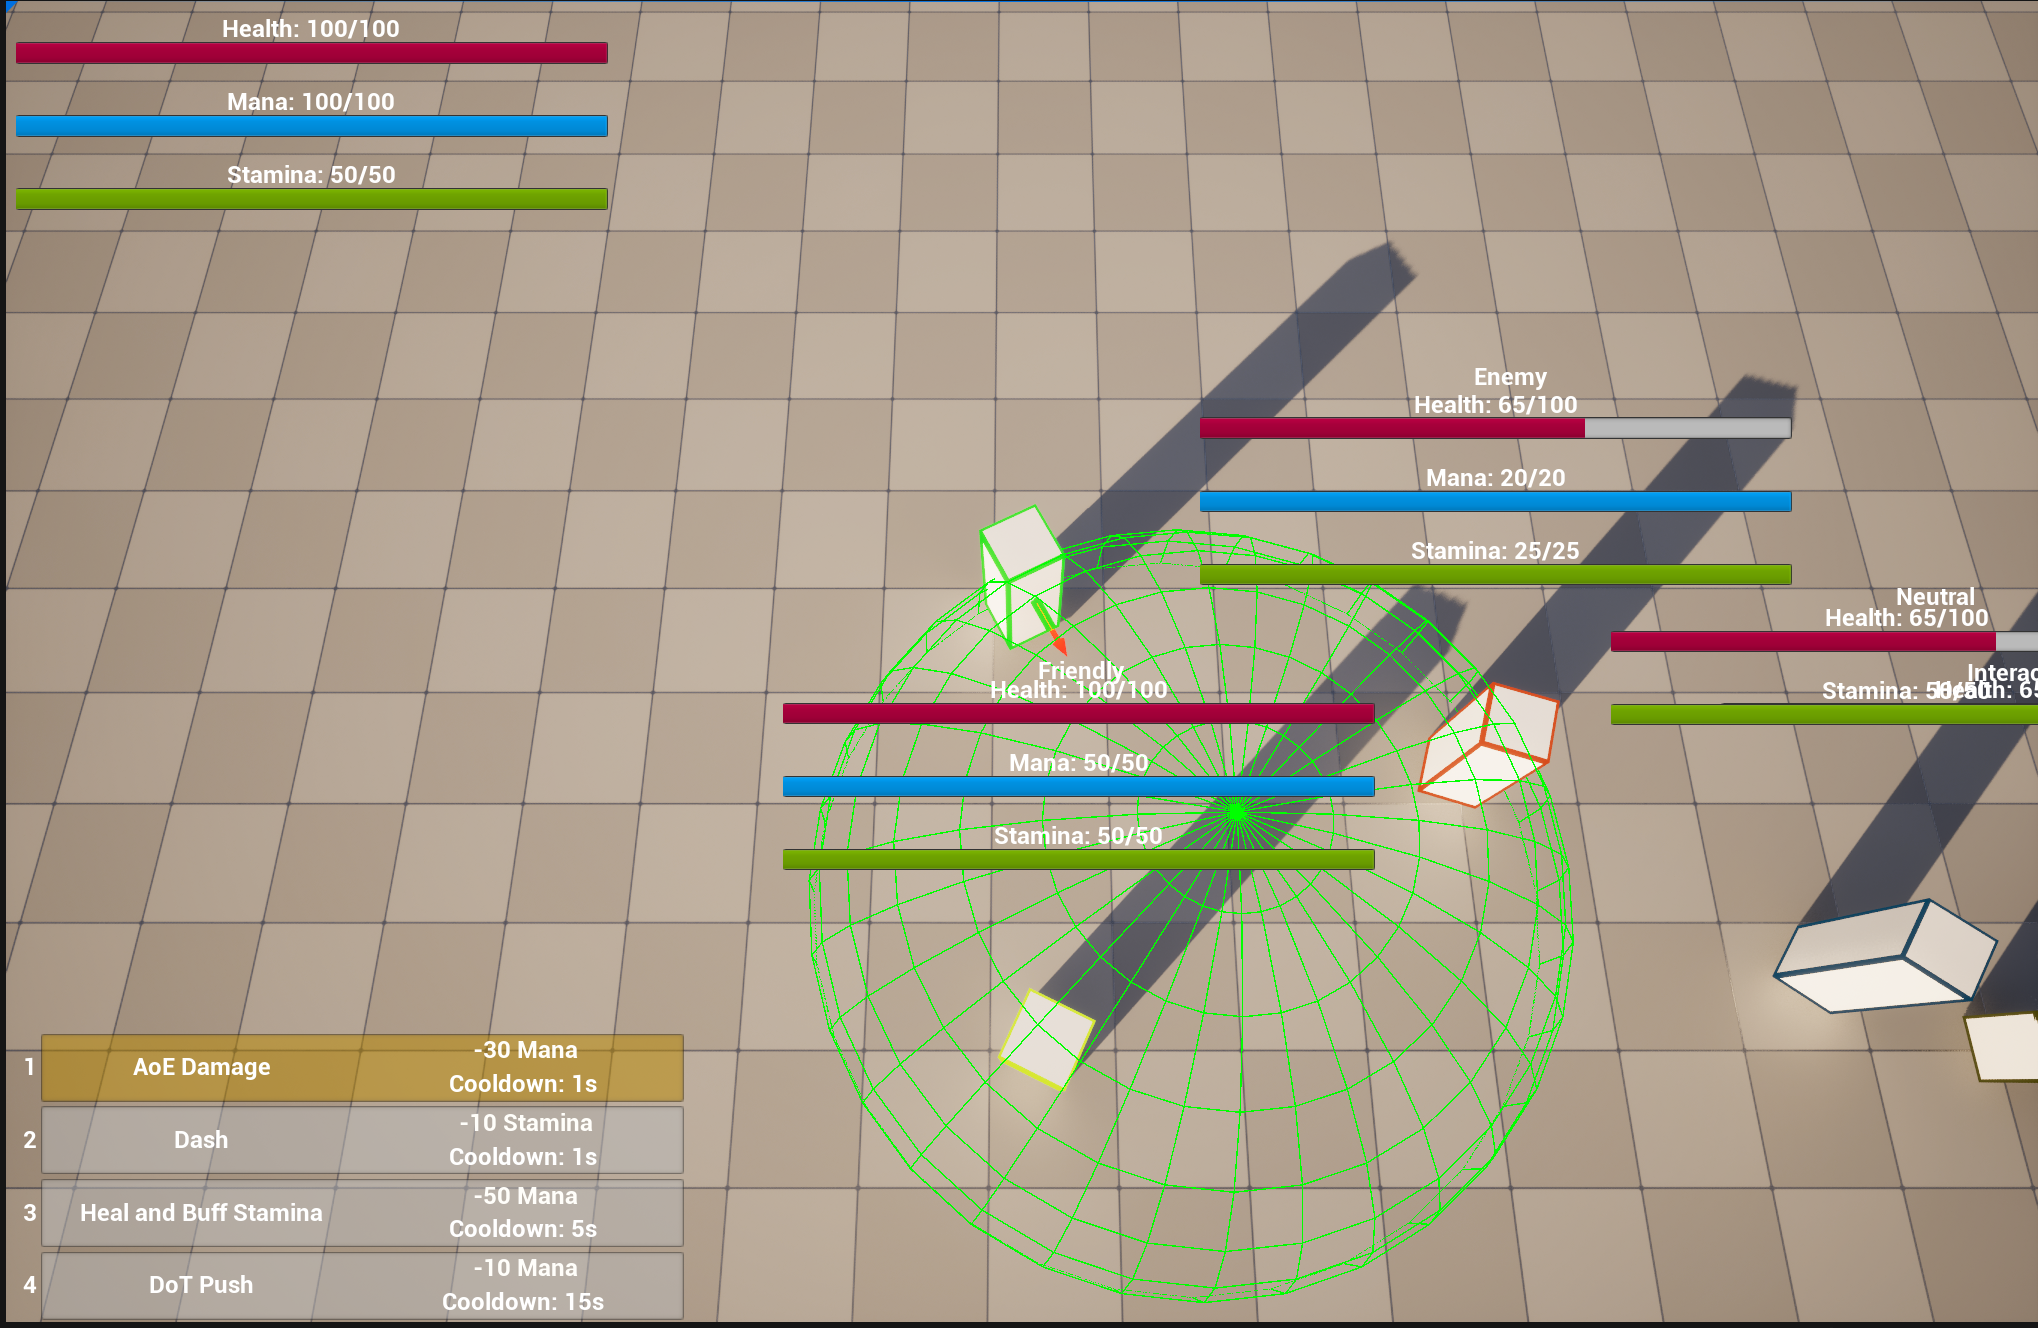
\includegraphics[width=.75\textwidth]{DemoRunning}
\caption*{\textit{The ability system running in Unreal Engine 5.}}
     \end{figure}

\vfill
            
\vspace{0.7cm}

       
Department of Computing\\
       Goldsmiths, University of London\\
\vspace{0.7cm}
\today
            
\end{center}
\end{titlepage}
\section*{Links}
Video: \url{https://youtu.be/cIZZLWoxqow}\\
GitHub Repository: \url{https://github.com/OdgeM/GameEnginesDemoProject}


\section{Introduction}

This project implements a modular ability and stat system inspired by action RPGs. The aim was to design a flexible framework where gameplay effects (i.e. damage, buffs, movement) can be defined independently and applied to different actors with varying capabilities. 
To achieve this, the system separates the data and behaviour of each component: thus, allowing for reusable and extensible gameplay logic. It draws from common practice in modern game development - particularly component-based architecture and effect-driven systems.
While the bulk of the core logic was implemented in C++, the goal was to allow for high-level customisation of abilities and stats from derived blueprints - therefore allowing less-technical designers to work with the system quickly and easily, without having to trawl through the source code.

\section{Program Overview}

The system allows actors to:
\begin{itemize}
    \item Possess a configurable set of stats (for the purposes of this demonstration, these are health, mana, and stamina)
    \item Execute abilities composed of modular effects
    \item Target abilities with a mouse-based system, while previewing the ability
    \item Apply ability outcomes on click
\end{itemize}

\section{Code List}


\section{Implementation}

\subsection{Stat System}

Stats are managed and modified for each actor within the \texttt{UStatComponent} class. Within this component, stats are stored within a \texttt{TMap<EStatsType, FStatData>}, where \texttt{EStatsType} is an enumerator which stores the possible stat types and \texttt{FStatData} is a struct which contains the current value and maximum value of each stat. 
Access to the stats is handled via Blueprint-callable functions, which follow a “bool and out” parameter pattern: whereby the function returns a bool if the operation was a success, and a parameter that is passed by reference returns the result - with the aim of safely handling missing stats.

\subsection{Stat Modifiers}

Modifications to stats utilise the \texttt{FStatModifier} struct. This struct contains:
\begin{itemize}
    \item The target stat, as an \texttt{EStatsType} value
    \item The operation to apply to the stat, defined by the \texttt{EModifierOp} enum - which contains “Add”, “Multiply” and “Override” options
    \item The magnitude of the operation to apply to the stat’s current value, as a float
    \item The magnitude of the operation to apply to the stat’s maximum value, as a float
    \item Two Boolean behaviour flags: 
    \begin{itemize}
        \item \texttt{bOverTime}: Whether the change should be applied over time
        \item \texttt{bTemporary}: Whether this is a temporary change that should be reverted
    \end{itemize}
    \item And a float which defines the duration of the effect if either of the above Booleans are true.
\end{itemize}

Stat changes are then centralised in the \texttt{UStatComponent::ApplyModifier} function, which ensures that there is only a single source of truth for the stat logic. Effects over time and temporary effects are handled using timers, which allows for multiple overlapping effects.

\subsection{Regeneration}

To have the actor passively regenerate stats for features like automatic health or mana regeneration, the component also contains a \texttt{RegenRate} member - which is a \texttt{TMap<EStatsType, float>} containing how much of that stat should be regenerated per second. 

\subsection{Abilities}

Abilities are managed by the \texttt{UAbilityComponent} class, which stores an array of the current abilities and handles the logic for adding, selecting, targeting, and activating those abilities.
Abilities are represented by the \texttt{UAbility} class which contains the following Blueprint-editable member variables, which can be used to configure the ability:
\begin{itemize}
    \item \texttt{FString Name}: The name of the ability to be used in the UI.    
    \item \texttt{TArray<UAbilityEffect*> Effects}: The effects of the ability.
    \item \texttt{UAbilityTargeting* TargetingStrategy}: How the ability is targeted. 
    \item \texttt{int32 TargetableTeams}: The “teams” that the ability can target (i.e. allies/enemies etc.)
    \item \texttt{float Cooldown}: How long it takes for the ability to cooldown.
    \item \texttt{TArray<UAbilityEffect*> Costs}: The stat costs required to activate the ability.
\end{itemize}

\subsection{Ability Effects}

The \texttt{UAbilityEffect} class is used to define the effects that an ability has. The main \texttt{UAbilityEffect} just contains an empty \texttt{Apply} function, which is overridden by subclasses to define custom logic. This allows for custom logic to be implemented as needed, without requiring any changes to the overall system structure. 
For this demonstration, three example effects were implemented:
\begin{itemize}
    \item \texttt{UStatEffect}: Applies an array of \texttt{FStatModifiers} to the target actors which is used for any effect that requires stat changes (i.e. damage, healing, buffs etc.).
    \item \texttt{UPushEffect}: Applies a force to the target actors to create a knockback effect.
    \item \texttt{UDashEffect}: Launches the instigating actor forwards.
\end{itemize}

\subsection{Ability Targeting}

Like effects, the targeting of abilities is handled by modular \texttt{UAbilityTargeting} classes which contains a \texttt{GetTargets} function which defines the targeting logic and an \texttt{UpdatePreview} function to update the visual effects previewing the ability in the game world. As with the effects, separating the targeting from the rest of the ability allows for high levels of extensibility and customisability. For this demonstration, the following targeting methods were created:
\begin{itemize}
    \item \texttt{USingleTargeting}: A single actor is targeted.
    \item \texttt{UAoETargeting}: All actors within a sphere are targeted.
    \item \texttt{UConeTargeting}: All actors within a cone in front of the instigating actor are targeted.
    \item \texttt{ULineTargeting}: All actors within a line in front of the instigating actor are targeted.
\end{itemize}

Targeting data is contained within the \texttt{FAbilityTargetingData} struct. This struct contains:
\begin{itemize}
    \item \texttt{AActor* HoverActor}: The actor currently underneath the mouse.
    \item \texttt{TArray<AActor*>}: The actors that are targeted by the ability.
    \item \texttt{FVector TargetLocation}: The world location that is being targeted.
    \item \texttt{FVector SourceLocation}: The world location where the effect will originate from.
\end{itemize}

The targeting data is passed by reference to the \texttt{GetTargets} function, which modifies the members as defined by its logic. This is then passed to the \texttt{UAbilityEffect} belonging to the ability, to define where the effect is applied.

\subsection{Teams and the Targetable Interface}

To allow different abilities to target different types of actors, an \texttt{ETeam} enum is used to define the possible “teams” that the actors belong to. For this demonstration these are:
\begin{itemize}
    \item Player
    \item Enemy
    \item Neutral
    \item Friendly
    \item Interactable
\end{itemize}

To allow an ability to target combinations of these, and to make this easy to use within Blueprints, this is used as a bitmask within the \texttt{UAbility} class - which creates a nice checkbox list within the editor.

To define which actors are targetable, a “Targetable” interface was implemented with a function to get the owner’s team and to set the owner as “targeted”. During targeting, actors are filtered by this interface, and the \texttt{UAbility} then further filters which actors belong to the targeted teams.

\subsection{Previewing Abilities}

Each \texttt{UAbilityTargeting} class contains logic to display an ability preview in the world - such as drawing a sphere for \texttt{UAoETargeting}. To further aid with targeting, the level contains a post-processing volume with a custom material which adds an outline to actors while targeting - with the colour representing their team (or black when not targetable), and the outline glowing brighter when that actor is targeted.

\subsection{Input System}

A \texttt{UPlayerController} subclass was created to handle the inputs for ability selection and activation. Using InputActions, abilities can be selected with the number keys which starts targeting. While targeting, the player controller casts a raycast at current mouse position, using the hit location and hit actor to constructs a \texttt{FAbilityTargetingData} struct - which is then passed by reference to the ability to allow the targeting strategy to populate the target actors and display the preview.

While targeting, left click activates the current ability, pressing a different number key changes the current ability, and pressing the same number key again deselects the current ability. If left click is pressed while no ability is selected, the character moves to the clicked position.

\subsection{UI}

A minimal UI was designed to demonstrate that the widget blueprints can interact with the C++ classes, retrieving stats and ability information.

\section{Problem Solving}

\subsection{Stacking Effects}

For effects applied over time, stacking multiple effects with different durations and magnitudes proved difficult. As mentioned, this was handled by using timers, which apply repeated modifiers over time and then automatically clear when the duration expires. This required that \texttt{FTimerHandle} for each effect had to be stored and identifiable - even after they were out of scope as otherwise, they would never be cleared. To solve this, \texttt{TSharedRef} shared handles were used to provide dynamic pointers to the handle which can then be captured in the timer lambda function.

\subsection{Outline Material}

As the post-processing material that applies the actor outlines during targeting was in a volume covering the whole play space, changing the outline colour of individual actors based on their team and whether they are targeted was a challenge. Simply modifying a parameter on the material would apply the change to all actors so, instead, custom depth stencils were used to encode the information.

Custom depth was already being used within the material to define the areas to apply outlines to, so using stencil values proved to be a natural extension. While the stencil values could be hard coded for each team used in this demonstration, this lacks the extensibility that this system is aiming for. Instead, the actor’s team was used as the stencil value and, as each actor can only belong to one team, the colour could be selected based on that - with the stencil value being equal to 2 raised to the power of the team’s position in the \texttt{ETeam} enum. However, to enable the outline to glow brighter when targeted, this proved insufficient. 

To encode the targeting information, the bit-wise representation of the \texttt{ETeam} value was considered. In this example, the \texttt{ETeam} value was represented in the five lowest bits of the 32-bit integer - with each bit representing a different team. For example, the value for “friendly” would be:

0 \quad 1 \quad 0 \quad 0 \quad 0

Interactable \quad Friendly \quad Neutral \quad Enemy \quad Player

As the additional information was just a Boolean value, only a single additional bit would be required. Therefore, the team value was bit-shifted left, and the new rightmost bit was used as a flag indicating if the actor was being targeted. In integer arithmetic, this process is equivalent to multiplying the integer team value by two and adding one if the actor is being targeted.

Then, using this as the stencil value, the material can then retrieve the original team value by dividing the stencil value by two and taking the floor of the new value - which is then used to select the correct colour. The targeting status is then decoded by taking checking if the remainder of the stencil value division is 0.5 or 0. If it is 0.5, then the bit flag was enabled and the actor is being targeted and, therefore, the brightness of the outline is increased.

\section{Future Work}

Several potential extensions could significantly improve both the flexibility and robustness of this system.

\subsection{Advanced Effect Stacking and Management}

The current system enables multiple effects to run simultaneously but lacks any formal stacking rules. Future work could introduce:
\begin{itemize}
    \item Stacking policies (e.g. refresh duration, accumulate intensity, or replace existing effects) 
    \item Effect identification IDs to track and manage individual instances 
    \item Priority systems for conflicting modifiers 
\end{itemize}

This would ensure that the effects interact predictably.

\subsection{Data-Driven Ability Design}

Currently, abilities and effects are defined in code or Blueprint classes. This could be improved by introducing:
\begin{itemize}
    \item DataAssets or data tables to define abilities externally 
    \item Designer-friendly configuration without recompilation 
    \item Easier balancing and iteration 
\end{itemize}

This would improve the scalability greatly, as it would further separate game logic from content.

\subsection{Visual Effects and UI Improvements}

The current UI is extremely barebones, and abilities lack visual effects altogether. Adding the option to configure abilities with casting and impact VFX and UI details (such as icons) would greatly improve the system.

\end{document}